\chapter{Relatividad General}
\label{cap:2}
\newpage

\section{Gravedad}

Luego de sus contribuciones sobre el estudio de los cuerpos a velocidades relativistas y de establecer una nueva formulación para la teoría electromagnética clásica consistente con sus aportes en Relatividad Especial, se había generado a su vez un nuevo problema: ¿cómo introducir la interacción gravitacional en su nueva teoría?.

No fue si no hasta 10 años después, en 1915, cuando en su trabajo titulado \textit{Grundgedanken der allgemeinen Relativitätstheorie und Anwendung dieser Theorie in der Astronomie} \cite{Einstein-2} (``Idea básica de la teoría general de la relatividad y aplicación de esta teoría en astronomía''), Einstein plantea una nueva forma de entender la gravedad, dicha formulación se conoce como \textbf{la Teoría de la Relatividad General}. 

Esta teoría está basada principalmente en un principio (postulado por el mismo Einstein), el cual nos dice que \textit{``El movimiento de un cuerpo producto de un campo gravitacional depende únicamente de su posición inicial en el espaciotiempo, no de su constitución. Y el resultado de cualquier experimento local, gravitacional o no, en un laboratorio en caída libre todos los efectos de la gravedad desaparece''}. Este principio recibe el nombre de \textbf{Principio de equivalencia fuerte} y plantea que, básicamente, no hay diferencia entre la gravedad provocada por la masa de los cuerpos, y los efectos de los sistema de referencia no inerciales\footnote{\url{http://teoria-de-la-relatividad.blogspot.com/2009/03/8-el-principio-de-equivalencia.html}} como se muestra en la figura \ref{fig:5}. Cabe mencionar que existe otro principio muy similar llamado \textbf{Principio de equivalencia débil}, el cual fue planteado por Galileo y nos dice que \textit{el movimiento de cualquier partícula de prueba en caída libre es independiente de su composición y estructura}. Comúnmente, este principio es utilizado para explicar el porqué los cuerpos en el vacío siempre caen con la misma aceleración, independiente de su masa.
\begin{figure}[!ht]
\centering
\begin{subfigure}{0.3\textwidth}
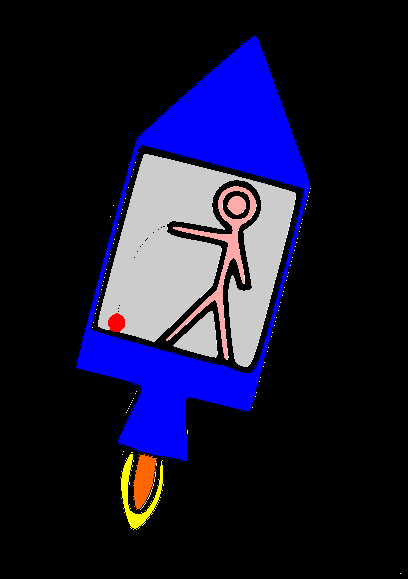
\includegraphics[width=\textwidth]{images/principio-equivalencia-1.pdf}
\caption{Cohete}
\end{subfigure}
\begin{subfigure}{0.3\textwidth}
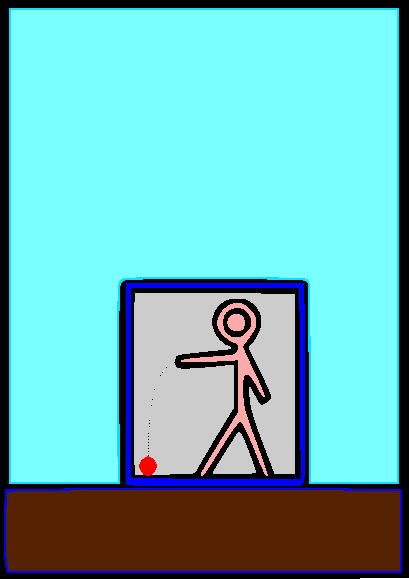
\includegraphics[width=\textwidth]{images/principio-equivalencia-2.pdf}
\caption{Tierra}
\end{subfigure}
\caption[Principio de equivalencia de Einstein]{Esquema explicativo del principio de equivalencia propuesto por Einstein.}
\label{fig:5}
\end{figure}

Una de las primeras predicciones de dicha teoría fue el cálculo del ángulo de deflexión de un haz de luz al pasar una distancia $R$ de un cuerpo central, efecto que fue verificado en 1919 a mano de Arthur Eddingon \textit{et.al.} \footnote{\url{https://es.wikipedia.org/wiki/Arthur_Stanley_Eddington/media/Archivo:1919_eclipse_positive.jpg}} \cite{Coles} (ver \ref{fig:6}), siendo éste uno de los primeros grandes avances sobre esta nueva forma de entender la gravedad.
\begin{figure}[!ht]
\centering
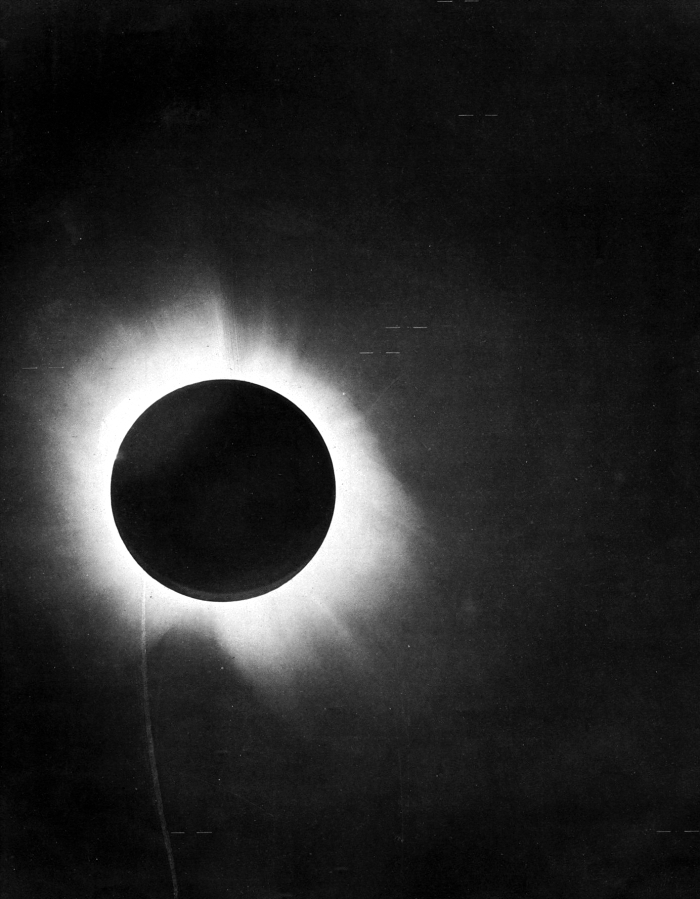
\includegraphics[scale=0.5]{images/1919eclipse.jpg}
\caption[Fotografía tomada por Eddintong]{Fotografía original tomada por Eddintong en 1919.}
\label{fig:6}
\end{figure}

\section{Ecuaciones de campo}
\label{sec:3}

Una de las razones principales de porqué Einstein tardó tanto en completar su teoría fue la necesidad de estudiar los avances en \textbf{Geometría diferencial}, área de las Matemáticas que se dedica al estudio de la geometría utilizando diversas herramientas del cálculo y álgebra. Los principales objetos de estudio en esta disciplina son las variedades diferenciales las cuales, principalmente, representan un espacio topológico que localmente se reduce al espacio Euclidiano.

Siendo más específico, Einstein se centró en el estudio de la geometría riemanniana para desarrollar su teoría, el cual tiene como elemento principal la \textbf{métrica}. Dicho elemento matemático nos permite definir el concepto de distancia y es representado por una matriz simétrica de $4 \cross 4$ con elementos reales.

Einstein logra asociar dicho elemento matemático a una propiedad intrínseca del espaciotiempo y muestra cómo la métrica es determinada por los elementos que conforman el espacio (energía), y el cómo la métrica a su vez determina la trayectoria de los objetos que se mueven en dicho espaciotiempo, dando origen a la famosa frase \textit{La materia le dice al espacio cómo curvarse, y el espacio le dice a la materia cómo moverse}\footnote{\url{https://es.wikiquote.org/wiki/John_Archibald_Wheeler}}.

Esta relación viene determinada por un conjunto de 10 ecuaciones diferenciales parciales no-lineales llamadas las ecuaciones de campo de Einstein,
\begin{equation}
\label{eq:7}
R_{\mu \nu} - \frac{1}{2}R g_{\mu \nu} = 8\pi  T_{\mu \nu},
\end{equation}
donde $R_{\mu \nu}$ es el tensor de Ricci, $R$ el escalar de curvatura, $g_{\mu \nu}$ la métrica del espaciotiempo, $T_{\mu \nu}$ el tensor de energía-momentum, $G$ la constante de gravitación universal y $c$ la velocidad de la luz en el vacío (ver Apéndice \ref{ape:convenciones}).

\subsection{Solución de Kerr}

La primera solución exacta de \eqref{eq:7} fue encontrada el año 1916 por el físico alemán Karl Schwarzschild (1873-1916) \cite{Heinicke}, dicha solución muestra cómo es la métrica al rededor de una distribución de masa $M$ esféricamente simétrica no-rotante, muchos nuevos conceptos son introducidos con esta nueva solución, como lo son el radio de Schwarzschild y el horizonte de eventos.

No fue hasta 1963 cuando el físico neozelandés Roy Kerr (1934-ahora) \cite{Heinicke} logra encontrar una nueva solución exacta a \eqref{eq:7}, la cual muestra cómo es la métrica fuera agujero negro rotante de masa $M$ y momento angular $J$, la cual es (en coordenadas de Boyer-Lindquist y expresada en términos de su elemento de línea)
\begin{equation}
\label{eq:8}
\mathrm{d}s^2 = \frac{\Delta}{\rho^2} \left( \mathrm{d}t - a \sin^2 \theta \mathrm{d}\phi \right)^2 - \frac{\sin^2 \theta}{\rho^2} \left[ (r^2 + a^2)\mathrm{d}\phi - a\mathrm{d}t \right]^2 - \frac{\rho^2}{\Delta} \mathrm{d}r^2 - \rho^2 \mathrm{d}\theta^2,
\end{equation}
donde: 
\begin{equation}
\rho^2 := r^2 + a^2 \cos^2 \theta ,\quad \Delta := r^2 - 2r + a^2, \quad m := GM, \quad a := \frac{J}{M}.
\end{equation}

Las principales propiedades de esta métrica son que es estacionaria y axialmente simétrica, de lo cual se puede inferir que hay dos vectores de Killing los cuales son $\partial_t$ y $\partial_{\phi}$, y por último, que la métrica es invariante bajo la transformación
\begin{eqnarray*}
t &\longrightarrow & -t ,\\
\phi &\longrightarrow & -\phi,
\end{eqnarray*} 

\section{Ecuación de desvío geodésico}

Como se muestra en la sección \ref{sec:1}, el estudio de las inhomogeneidades del campo gravitacional newtoniano y el campo electromagnético determinan las fuerzas de marea. En el contexto de Relatividad General es posible estudiar el mismo problema.

Consideremos $g_{\mu \nu}$ como la métrica del espaciotiempo, y consideremos una trayectoria parametrizada por $x^{\mu}(s)$. Se define la derivada covariante de $A^{\mu}$ sobre la curva como
\begin{equation}
\label{eq:9}
\cd{A^{\mu}} := \dv{A^{\mu}}{s} + \Gamma^{\mu}_{\rho \sigma} \dv{x^{\rho}}{\s} A^{\sigma},
\end{equation}
donde $s$ es un parámetro afín, $\Gamma^{\mu}_{\rho \sigma}$ son los símbolos de Christoffel de segunda especie (ver Apéndice \ref{ape:convenciones}). 

Se puede ver que si $x^{\mu}(s)$ es una geodésica, entonces
\begin{equation}
\cd{ } \left[ \dv{x^{\mu}}{\s} \right] = 0.
\end{equation} 

\begin{lemma}
\label{lema:1}
Sean $G_1$ y $G_2$ dos geodésicas parametrizadas por el mismo parámetro afín $s$ y separadas una distancia infinitesimal, si $x^{\mu}_1(s)$ y $x^{\mu}_2(s)$ son las parametrizaciones de ambas geodésicas respectivamente, y se define la 4-velocidad como $u^{\mu}(s) := \mathrm{d}x^{\mu}_1/\mathrm{ds}$, entonces la segunda derivada covariante sobre la curva $x^{\mu}_1$ de $\delta x^{\mu}:= x^{\mu}_2 - x^{\mu}_1$ es
\begin{equation}
\label{eq:10}
\frac{\delta^2}{\mathrm{ds}^2}\delta x^{\mu} = \dv[2]{\delta x^{\mu}}{\s} + \partial_{\nu} \Gamma^{\mu}_{\rho \sigma} u^{\rho} u^{\sigma} \delta x^{\nu} - R^{\mu}_{\ \rho \sigma \nu} u^{\rho} u^{\nu} \delta x^{\sigma} + 2 \Gamma^{\mu}_{\sigma \rho} u^{\sigma} \dv{ }{\s} \delta x^{\rho}, 
\end{equation}
donde $R^{\mu}_{\ \rho \sigma \nu}$ es el tensor de Riemann.
\end{lemma}
\begin{proof}

De \eqref{eq:9} sabemos que
\begin{align}
\frac{\delta^2}{\mathrm{ds}^2}\delta x^{\mu} &= \cd{ } \left[ \cd{ } \delta x^{\mu} \right] \nonumber \\
&= \dv{ }{\s} \left[ \cd{ } \delta x^{\mu} \right] + \Gamma^{\mu}_{\rho \sigma} u^{\rho} \cd{ } \delta x^{\sigma} \nonumber \\
\label{eq:81}
&= \dv[2]{ }{\s} \delta x^{\mu} + \dv{ }{\s} \left[ \Gamma^{\mu}_{\rho \sigma} u^{\rho} \delta x^{\sigma} \right] + \Gamma^{\mu}_{\rho \sigma} u^{\rho} \dv{ }{\s}\delta x^{\sigma} + \Gamma^{\mu}_{\rho \sigma} \Gamma^{\sigma}_{\alpha \beta} u^{\rho} u^{\alpha} \delta x^{\beta}.
\end{align}

El segundo término en \eqref{eq:81} puede ser escrito como
\begin{equation}
\label{eq:11}
\dv{ }{\s} \left[ \Gamma^{\mu}_{\rho \sigma} u^{\rho} \delta x^{\sigma} \right]
=
\left( \dv{ }{\s} \Gamma^{\mu}_{\rho \sigma} \right) u^{\rho} \delta x^{\sigma} + \Gamma^{\mu}_{\rho \sigma} \left(  \dv{ }{\s} u^{\rho} \right) \delta x^{\sigma} + \Gamma^{\mu}_{\rho \sigma} u^{\rho} \left( \dv{ }{\s} \delta x^{\sigma} \right).
\end{equation}

Además, por la regla de la cadena sabemos que
\begin{equation}
\label{eq:12}
\dv{ }{\mathrm{s}} \Gamma^{\mu}_{\rho \sigma} = \partial_{\lambda} \Gamma^{\mu}_{\rho \sigma} u^{\lambda},
\end{equation}
y, como $x_1^{\mu}(s)$ es una geodésica,
\begin{equation}
\label{eq:13}
\dv{u^{\mu}}{\mathrm{s}} + \Gamma^{\mu}_{\rho \sigma} u^{\rho} u^{\sigma} = 0.
\end{equation}

Reemplazando \eqref{eq:12} y \eqref{eq:13} en \eqref{eq:11},
\begin{equation}
\label{eq:14}
\dv{ }{\s} \left[ \Gamma^{\mu}_{\rho \sigma} u^{\rho} \delta x^{\sigma} \right]
=
\partial_{\lambda} \Gamma^{\mu}_{\rho \sigma} u^{\rho} \delta x^{\sigma} - \Gamma^{\mu}_{\rho \sigma} \Gamma^{\rho}_{\alpha \beta} u^{\alpha} u^{\beta} \delta x^{\sigma} + \Gamma^{\mu}_{\rho \sigma} u^{\rho} \dv{ }{\s} \delta x^{\sigma}.
\end{equation}

Luego, \eqref{eq:14} en \eqref{eq:81},
\begin{equation}
\label{eq:15}
\frac{\delta^2}{\mathrm{ds}^2}\delta x^{\mu} = \dv[2]{ }{\mathrm{s}} \delta x^{\mu} + 
\left[ \partial_{\sigma} \Gamma^{\mu}_{\rho \nu} + \Gamma^{\mu}_{\delta \sigma} \Gamma^{\delta}_{\rho \nu} - \Gamma^{\mu}_{\delta \nu} \Gamma^{\delta}_{\rho \sigma}  \right] u^{\rho} u^{\sigma} \delta x^{\nu} + 2\Gamma^{\mu}_{\alpha \beta} u^{\alpha} \dv{ }{\mathrm{s}} \delta x^{\nu}.
\end{equation}

Por la definición del tensor de Riemann \ref{ape:convenciones} se puede ver que
\begin{equation}
\label{eq:16}
R^{\mu}_{\ \nu \rho \sigma} + \partial_{\sigma} \Gamma^{\mu}_{\rho \rho} = \partial_{\rho} \Gamma^{\mu}_{\rho \sigma} + \Gamma^{\mu}_{\rho \delta} \Gamma^{\delta}_{\nu \sigma} - \Gamma^{\mu}_{\sigma \delta} \Gamma^{\delta}_{\nu \rho},
\end{equation}
así
\begin{equation}
\frac{\delta^2}{\mathrm{ds}^2}\delta x^{\mu} = \dv[2]{\delta x^{\mu}}{\s} + \left( \partial_{\nu} \Gamma^{\mu}_{\rho \sigma} \right) u^{\rho} u^{\sigma} \delta x^{\nu} - R^{\mu}_{\ \rho \sigma \nu} u^{\rho} u^{\nu} \delta x^{\sigma} + 2 \Gamma^{\mu}_{\sigma \rho} u^{\sigma} \dv{ }{\s} \delta x^{\rho},
\end{equation}
lo cual prueba el lemma.
\end{proof}

\begin{theorem}
\label{teo:1}
Sean $G_1$ y $G_2$ dos geodésicas parametrizadas por el mismo parámetro afín $s$, separadas infinitesimalmente, y si 
$$|\dv{ }{\s} \delta x^{\rho}| \ll |u^{\rho}(s)|$$
es decir, los vectores tangentes a las geodésicas definidos como $u^{\mu}_{1,2}(s) := \mathrm{d}x^{\mu}_{1,2}/\mathrm{ds}$ son aproximadamente iguales. Entonces la segunda derivada covariante a lo largo de $x^{\mu}_1$ de $\delta x^{\mu}$ es
\begin{equation}
\label{eq:17}
\frac{\delta^2}{\mathrm{ds}^2}\delta x^{\mu} = - R^{\mu}_{\ \sigma \nu \rho} u^{\sigma} u^{\nu} \delta x^{\rho}.
\end{equation}
\end{theorem}
\begin{proof}
Para dos geodésicas se sabe que
\begin{equation}
\cd{ }\left[ \dv{x_1^{\mu}}{\mathrm{s}} \right] = \cd{ }\left[ \dv{x_2^{\mu}}{\mathrm{s}} \right] = 0,
\end{equation}
luego
\begin{equation}
\label{eq:18}
\dv[2]{x_1^{\mu}}{\mathrm{s}} + \Gamma^{\mu}_{\rho \sigma} \dv{x^{\rho}}{\mathrm{s}} \dv{x^{\sigma}}{\mathrm{s}} = 0,
\end{equation}
donde los símbolos de Christoffel están evaluados a lo largo de $x_1$. Para la segunda geodésica sabemos que $x_2^{\mu} = x_1^{\mu} + \delta x^{\mu}$, así
\begin{equation}
\label{eq:19}
\dv[2]{x_1^{\mu}}{\mathrm{s}} + \dv[2]{ }{\mathrm{s}} \delta x^{\mu} + \Gamma^{\mu}_{\rho \sigma} \dv{ }{\mathrm{s}} \left( x_1^{\rho} + \delta x^{\rho} \right) \dv{ }{\mathrm{s}} \left( x_1^{\sigma} + \delta x^{\sigma} \right) = 0,
\end{equation}
donde en este caso, los símbolos de Christoffel están evaluados a lo largo de $x_2=x_1 + \delta x$. 

Expandiendo hasta primer orden se obtiene que
\begin{equation}
\label{eq:20}
\Gamma^{\mu}_{\rho \sigma}[x + \delta x] = \Gamma^{\mu}_{\rho \sigma}[x] + \partial_{\nu} \Gamma^{\mu}_{\rho \sigma}[x] \delta x^{\nu} + \mathcal{O}(\delta x^2).
\end{equation}

Reemplazando \eqref{eq:20} en \eqref{eq:19}, encontramos que hasta primer orden en $\delta x$,
\begin{equation}
0 = \dv[2]{x_1^{\mu}}{\mathrm{s}} + \dv[2]{ }{\mathrm{s}} \delta x^{\mu} + \left( \Gamma^{\mu}_{\rho \sigma}[x] + \left( \partial_{\nu} \Gamma^{\mu}_{\rho \sigma}[x] \right) \delta x^{\nu} \right) \dv{ }{\mathrm{s}} \left( x_1^{\rho} + \delta x^{\rho} \right) \dv{ }{\mathrm{s}} \left( x_1^{\sigma} + \delta x^{\sigma} \right).
\end{equation}

Luego, definiendo $u^{\mu} := \mathrm{d} x^{\mu}_1 / \mathrm{ds}$,
\begin{equation}
\label{eq:21}
0 = \dv[2]{x_1^{\mu}}{\mathrm{s}} + \dv[2]{ }{\mathrm{s}} \delta x^{\mu} + \Gamma^{\mu}_{\rho \sigma} u^{\rho} u^{\sigma} + \left( \partial_{\lambda} \Gamma^{\mu}_{\rho \sigma} \right) u^{\rho} u^{\sigma} \delta x^{\lambda} + 2 \Gamma^{\mu}_{\rho \sigma} u^{\rho} \dv{ }{\mathrm{s}} \delta x^{\sigma}. 
\end{equation}

Así, reemplazando \eqref{eq:18} en \eqref{eq:21} se deduce que
\begin{equation}
0 = \dv[2]{ }{\mathrm{s}} \delta x^{\mu} + \partial_{\lambda} \Gamma^{\mu}_{\rho \sigma} u^{\rho} u^{\sigma} \delta x^{\lambda} + 2 \Gamma^{\mu}_{\rho \sigma} u^{\rho} \dv{ }{\mathrm{s}} \delta x^{\sigma}.
\end{equation}

Finalmente, usando el lema \ref{lema:1} encontramos que
\begin{equation}
\frac{\delta^2}{\mathrm{ds}^2}\delta x^{\mu} = - R^{\mu}_{\ \sigma \nu \rho} u^{\sigma} u^{\nu} \delta x^{\rho},
\end{equation}
lo cual prueba el teorema.
\end{proof}

La ecuación \eqref{eq:17} describe las inhomogeidades de la curvatura y es conocida como la \textbf{ecuación de desvío geodésico} \cite{Ciufolini}.

\section{Campos gravitacionales débiles}

Como se dijo en la sección \ref{sec:3}, las ecuaciones de campo de Einstein son no-lineales en la métrica, y por ende, sus soluciones no dependen linealmente del tensor energía-momentum. Además, como dicho tensor, el cual se encuentra en el lado derecho de \eqref{eq:7} está multiplicado por $G$, entonces las soluciones dependerán no-linealmente de $G$.

Es bien sabido que la solución de ecuaciones no-lineales es un área de las matemáticas de difícil estudio, puesto que al no ser lineales, no existen métodos generales para poder resolverlas. Es por esto que se han desarrollado métodos aproximados para resolver dichas ecuaciones, en particular, es posible utilizar un método perturbativo para determinar las soluciones de \eqref{eq:7} como una serie infinita de términos.

Si usamos coordenadas pseudo-euclidianas y consideramos pequeñas perturbaciones de la forma
\begin{equation}
g_{\mu \nu} = \eta_{\mu \nu} + h_{\mu \nu}, \qquad |h_{\mu \nu}| \leq 1,
\end{equation}
donde $\eta_{\mu \nu} = \mathrm{diag}(1,-1,-1,-1)$ corresponde a la métrica plana, y si separamos las perturbaciones en una serie de órdenes en potencias de G, se puede escribir que
\begin{equation}
\label{eq:120}
g_{\mu \nu} = \eta_{\mu \nu} + h_{\mu \nu}^{(1)} + h_{\mu \nu}^{(2)} + \dots.
\end{equation}

Además de hacer la expansión de la métrica en distintos órdenes en $h$, es posible realizar una expansión similar para cada cantidad relevante en geometría riemanniana, así
\begin{align}
\label{eq:116}
\Gamma^{\lambda}_{\mu \nu} &= \Gamma^{(1)\lambda}_{\mu \nu} + \Gamma^{(2)\lambda}_{\mu \nu} + \dots,\\
\label{eq:117}
R_{\mu \nu} &= R_{\mu \nu}^{(1)} + R_{\mu \nu}^{(1)} + \dots,\\
\label{eq:118}
G_{\mu \nu} &= G_{\mu \nu}^{(1)} + G_{\mu \nu}^{(2)} + \dots,\\
\label{eq:119}
T_{\mu \nu} &= T_{\mu \nu}^{(0)} + T_{\mu \nu}^{(1)} + \dots.
\end{align}

El primer término de los símbolos de Christoffel en \eqref{eq:116}, el tensor de Ricci en \eqref{eq:117} y el tensor de Einstein en \eqref{eq:118} son cero, puesto que al ser proporcionales a derivadas de la métrica, y como el primer orden en \eqref{eq:120} es constante, entonces estas cantidades comienzan del orden 1.

De esta forma, las ecuaciones de campo de Einstein se pueden escribir como
\begin{equation}
G_{\mu \nu}^{(1)} + G_{\mu \nu}^{(2)} + \dots = \frac{8 \pi G}{c^4} \left( T_{\mu \nu}^{(0)} + T_{\mu \nu}^{(1)} + \dots \right),
\end{equation}
que puede ser separada en distintos órdenes como
\begin{align}
G_{\mu \nu}^{(1)} &= \frac{8 \pi G}{c^4} T_{\mu \nu}^{(0)},\\
G_{\mu \nu}^{(2)} &= \frac{8 \pi G}{c^4} T_{\mu \nu}^{(1)},\\
G_{\mu \nu}^{(3)} &= \frac{8 \pi G}{c^4} T_{\mu \nu}^{(2)},\\
\nonumber
& \vdots
\end{align}

Note que siempre se asocia cada orden del tensor de Einstein, a un orden menor del tensor de energía-momentum. Esto es por que la expansión es en términos de $G$, y al haber un $G$ multiplicando a $T_{\mu \nu}$, entonces la combinación $GT_{\mu \nu}^{(0)}$ es de orden 1.

\subsection{Expansión a primer orden}
\subsubsection{Métrica inversa}

A primer orden en $G$ se tiene que la métrica del espaciotiempo adpota la forma de
\begin{equation}
g_{\mu \nu} = \eta_{\mu \nu} + h_{\mu \nu}^{(1)},
\end{equation}
por convención, se suben y bajan los índices usando la métrica plana.

La primera cantidad necesaria a obtener es la métrica inversa, usando la propiedad que $\delta^{\mu}_{\nu} = g^{\mu \lambda} g_{\nu \lambda}$, y que
\begin{equation}
g^{\mu \nu} = \eta^{\mu \nu} + g^{\mu \nu}_{(1)} + \mathcal{O}(G^2),
\end{equation}
se obtiene que 
\begin{equation}
g^{\mu \nu}_{(1)} = -h^{\mu \nu}_{(1)} := -\eta^{\mu \lambda} \eta^{\nu \rho} h_{\lambda \rho}^{(1)}.
\end{equation}

\subsubsection{Conexión}
A primer orden, el primer término en la serie de los símbolos de Christoffel es:
\begin{equation}
\Gamma^{(1)\lambda}_{\mu \nu} = \frac{1}{2} \left( \partial_{\mu} h^{\lambda}_{(1) \nu} + \partial_{\nu} h^{\lambda}_{(1) \mu} - \partial^{\lambda} h_{\mu \nu}^{(1)} \right).
\end{equation}

\subsubsection{Tensor de Riemann}
Por otra parte, el primer orden del tensor de curvatura es:
\begin{equation}
\label{eq:85}
R^{\rho}_{(1) \mu \nu \lambda} = \frac{1}{2} \left( \partial_{\mu} \partial_{\nu} h^{\rho}_{(1) \lambda} - \partial_{\mu} \partial_{\lambda} h^{\rho}_{(1) \nu} + \partial_{\lambda} \partial^{\rho} h_{\mu \nu}^{(1)} - \partial_{\nu} \partial^{\rho} h_{\mu \lambda}^{(1)} \right).
\end{equation}

A partir del tensor de Riemann, es posible contraer índices para obtener todas las demás cantidades subsecuentes, tales como el tensor de Ricci, el escalar de curvatura y el tensor de Einstein.

\section{Expansión multipolar en GR}

En Física los problemas siempre involucran cuerpos extendidos (con volumen), lo cual en muchos casos representa un gran problema matemático a la hora de trabajar ecuaciones. Por esta razón se definen cantidades como el centro de masa, punto al que se le asignan propiedades del sistema completo (como masa o velocidad). Si bien esta forma de trabajar simplifica el análisis, al ser solo una aproximación, algunos efectos no pueden ser descritos usando solo el centro de masa \cite{nataly}.

Algo similar ocurre en Relatividad General: si se desea estudiar el comportamiento de un cuerpo extendido sería necesario considerar un \textit{tubo de mundo} en vez de una \textit{línea de mundo} como usualmente se hace con partículas puntuales.

La idea a grandes rasgos es reemplazar el tubo de mundo $\Sigma$ por una línea de mundo $L$, y el tensor de energía-momentum $T^{\mu \nu}$ por un conjunto de momentos multipolares $t^{\mu \nu}, t^{\mu \nu \sigma}, t^{\mu \nu \sigma \lambda}, \cdots$ a lo largo de $L$ (ver figura \ref{fig:1}), y donde la ley de balance del tensor energía-momentum permite determinar la evolución de dichos momentos multipolares.
\begin{figure}[!ht]
	\centering
	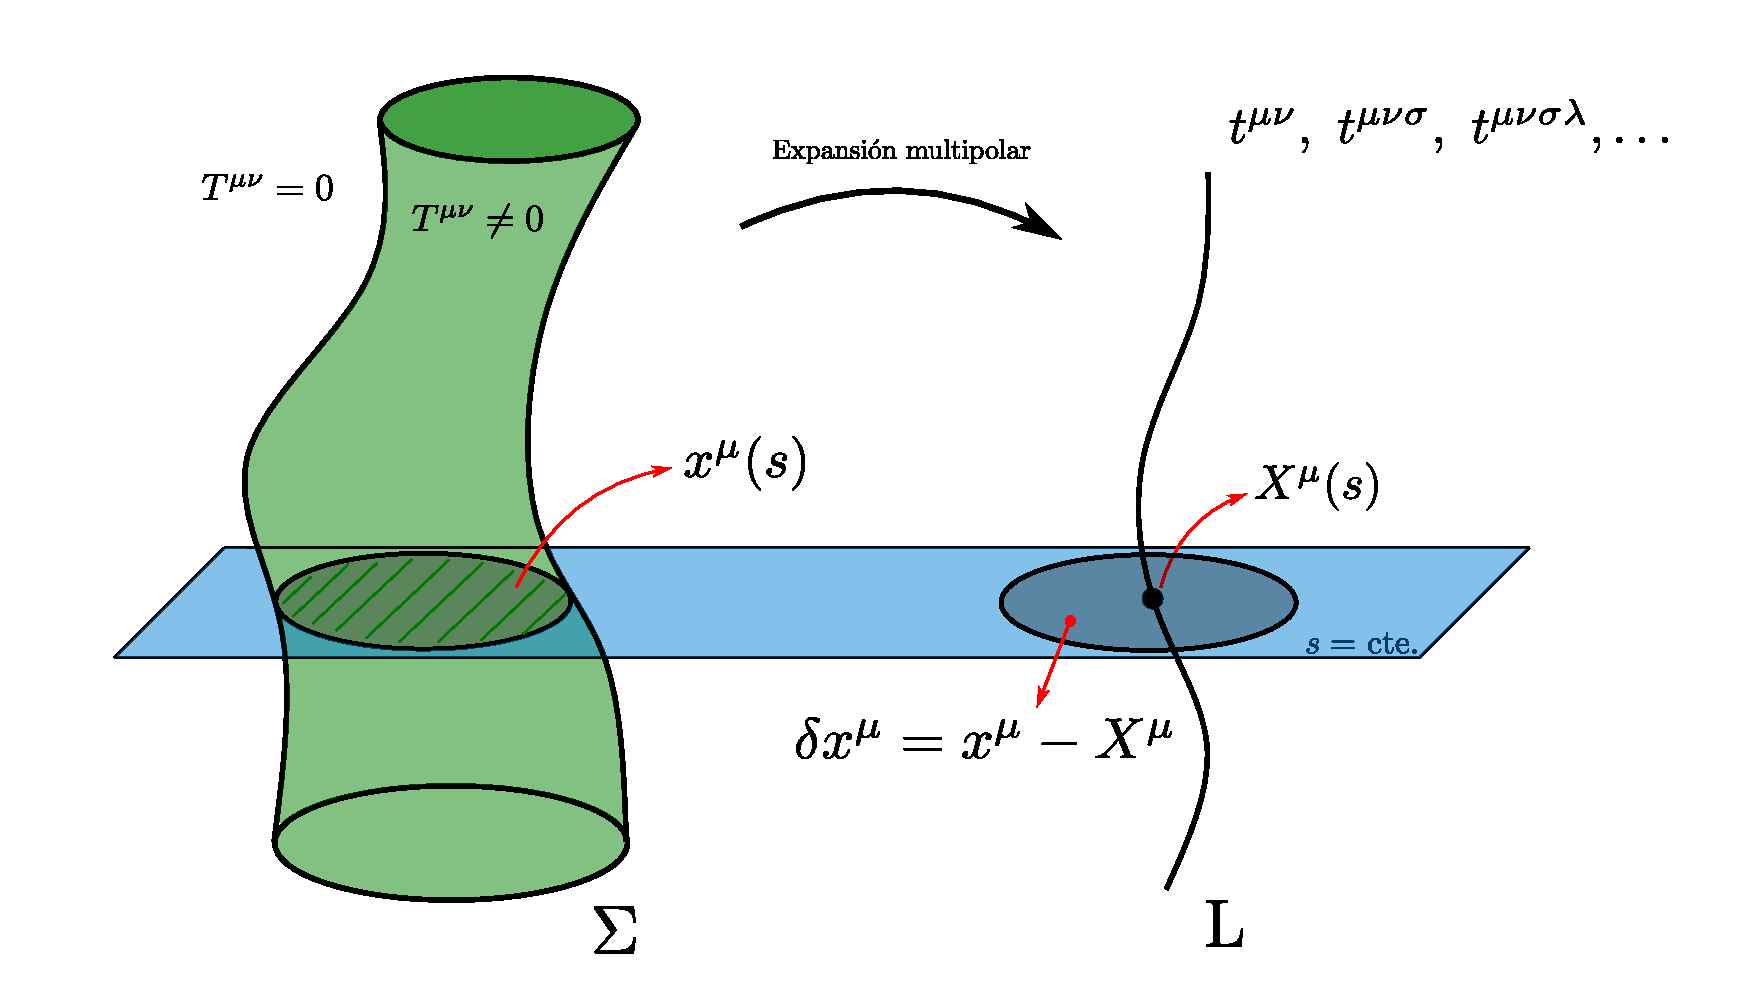
\includegraphics[scale=0.45]{images/papapetrou.pdf}
	\caption[Expansión multipolar en RG]{Esquema de la abstracción de tubo de mundo a línea de mundo}
	\label{fig:1}
\end{figure}
En el año 1951, el físico griego-francés Achille Papapetrou (1907-1997) en su trabajo titulado ``\textit{Spinning test-particles in general relativity. I}"" \cite{Papapetrou2,Papapetrou1} deriva por primera vez un método para obtener las ecuaciones de movimiento para cuerpos que poseen estructura interna, lo cual permitía introducir nuevas propiedades a dichos cuerpos como por ejemplo rotación interna (spin). 

Con el pasar de los años, se han desarrollado métodos alternativos para obtener las mismas ecuaciones sin los problemas que presentaban originalmente las ecuaciones de Papapetrou, entre los cuales destaca el carácter no-covariante de las ecuaciones de movimiento, esto por separar en el cálculo las componentes temporales y espaciales.

En \cite{Steinhoff-Puetzfeld} se utiliza la ecuación de conservación covariante del tensor de energía momentum
\begin{equation}
\label{eq:22}
\nabla_{\nu} T^{\mu \nu} = 0,
\end{equation}
de forma que se pueda escribir el tensor energía-momentum como la expansión en una serie de momentos multipolares, para luego obtener una conjunto de condiciones a satisfacer por los coeficientes de la expansión. De esta forma
\begin{align}
\nonumber
\tilde{T}^{\mu \nu} &= \int^{+\infty}_{-\infty} \left[ t^{\mu \nu} \delta_{(4)}(x^{\mu} - X^{\mu}(s)) + \nabla_{\lambda} [t^{\lambda \mu \nu} \delta_{(4)}(x^{\mu} - X^{\mu}(s))] \right.\\
&\quad \left.  + \nabla_{\rho} \nabla_{\lambda} [t^{\rho \lambda \mu \nu} \delta_{(4)}(x^{\mu} - X^{\mu}(s))] +  \dots
\right] \mathrm{d}s,
\end{align}
corresponde a la expansión de $\tilde{T}$, donde $t^{\mu \nu \dots}$ son los momentos multipolares, $\delta_{(4)}$ es la delta de Dirac 4-dimensional, $X^{\mu}(s)$ la parametrización de la curva de referencia que representa el tubo de mundo, y $s$ el parámetro afín con el cual se describe la curva. También es necesario mencionar que la cantidad que se escribe en términos de los momentos multipolares es la densidad tensorial de energía-momentum (ver Apéndice \ref{ape:convenciones}), esto es por la presencia de la delta de Dirac en su expansión.

También es necesario definir lo que en \cite{Tulczyjew} es llamada como \textit{forma canónica}. Se dice que una densidad tensorial arbitraria $\tilde{A}^{c_1 c_2 \dots}$ se encuentra en su forma canónica si puede ser escrita de la forma
\begin{equation}
\tilde{A}^{c_1 c_2 \dots} = \sum_{k=0}^{m} \int_{-\infty}^{+\infty} \nabla_{c_1 c_2 \dots c_k} \left[ \alpha^{c_1 \dots c_k b_1 \dots b_n} \delta_{(4)}(x^{\mu} - X^{\mu}(s)) \right], 
\end{equation}
donde los coeficientes satisfacen que
\begin{align}
\alpha^{c_1 \dots c_k b_1 \dots b_n} &= \alpha^{(c_1 \dots c_k) b_1 \dots b_n},\\
u_{c_1}\alpha^{c_1 \dots c_k b_1 \dots b_n} &= 0,
\end{align}
y se define el vector tangente a lo largo de la trayectoria como $u^{\mu} := \mathrm{d}X^{\mu} / \mathrm{d}s$.

\begin{theorem}
\label{teo:2}
Si para una densidad tensorial escrita en su forma canónica $\tilde{A}^{b_1 \dots b_n}$ y un arbitrario campo tensorial $T_{b_1 \dots b_n}$ se tiene que
\begin{equation}
\int_{\Omega}  \tilde{A}^{b_1 \dots b_n}T_{b_1 \dots b_n} = 0,
\end{equation}
en una región arbitraria del espaciotiempo $\Omega$, entonces todos los coeficientes de la expansión $\alpha^{c_1 \dots c_k b_1 \dots b_n}$ son nulos.
\end{theorem}

La demostración de este teorema puede encontrarse en \cite{Tulczyjew}.

\subsection{Descomposiciones respecto la velocidad}

Consideraremos que de forma general, los momentos multipolares satisfacen las siguientes simetrías:
\begin{equation}
t^{\lambda_1 \dots \lambda_n \mu \nu} = t^{\lambda_1 \dots \lambda_n (\mu \nu)}, \qquad t^{\lambda_1 \dots \lambda_n \mu \nu} = t^{(\lambda_1 \dots \lambda_n) \mu \nu}.
\end{equation}

Con ayuda del proyector $\rho^{\mu}_{\ \nu} := \delta^{\mu}_{\ \nu} - u^{\mu}u_{\nu}$, podemos hacer una descomposición de cada momento multipolar en términos de sus componentes ortogonales a $u^{\mu}$, recordando que $u^{\mu}u_{\mu} = 1$. Así, para el momento monopolar se tiene que
\begin{equation}
\label{eq:23}
t^{\mu \nu} = \ \des{0}{o}^{\mu \nu} + 2 \des{0}{o}^{(\mu} u^{\nu )} + \des{0}{t} u^{\mu} u^{\nu},
\end{equation}
donde
\begin{align*}
\des{0}{o}^{\mu \nu} &:=  \rho^{\mu}_{\ \lambda} \rho^{\nu}_{\ \sigma} t^{\lambda \sigma},\\
\des{0}{o}^{\mu} &:= \rho^{\mu}_{\ \lambda} u_{\nu} t^{\lambda \nu},\\
\des{0}{t} &:= t^{\mu \nu} u_{\mu} u_{\nu}.
\end{align*}

Para el momento dipolar se tiene que
\begin{equation}
\label{eq:24}
t^{\mu \nu \gamma} = \ \des{1}{o}^{\mu \nu \gamma} + 2 \des{1}{o}^{\mu ( \nu} u^{\gamma )} + \des{1}{o}^{\mu} u^{\nu} u^{\gamma} + u^{\mu} t^{\nu \gamma},
\end{equation}
donde
\begin{align*}
\des{1}{o}^{\mu \nu \gamma} &:= \rho^{\mu}_{\ \sigma} \rho^{\nu}_{\ \rho} \rho^{\gamma}_{\ \lambda} t^{\sigma \rho \lambda},\\
\des{1}{o}^{\mu \nu} &:= \rho^{\mu}_{\ \sigma} \rho^{\nu}_{\ \rho} u_{\lambda} t^{\sigma \rho \lambda},\\
\des{1}{o}^{\mu} &:= \rho^{\mu}_{\ \sigma} u_{\rho} u_{\lambda} t^{\sigma \rho \lambda},\\
\des{1}{t}^{\mu \nu} &:= t^{\lambda \mu \nu} u_{\lambda}.
\end{align*}

Y para el momento cuadrupolar se tiene que
\begin{equation}
\des{2}{t}^{\mu \nu \gamma \delta} = \ \des{2}{o}^{\mu \nu \gamma \delta} + 2 \des{2}{o}^{\mu \nu (\gamma} u^{\delta)} + \des{2}{o}^{\mu \nu} u^{\gamma} u^{\delta} - u^{\mu} u^{\nu} \des{2}{t}^{\gamma \delta} + 2 u^{(\mu} \des{2}{t}^{\nu) \gamma \delta},
\end{equation}
donde
\begin{align*}
\des{2}{o}^{\mu \nu \gamma \delta} &:= \rho^{\mu}_{\ \sigma} \rho^{\nu}_{\ \rho} \rho^{\gamma}_{\ \lambda} \rho^{\delta}_{\ \xi} t^{\sigma \rho \lambda \xi},\\
\des{2}{o}^{\mu \nu \gamma} &:= \rho^{\mu}_{\ \sigma} \rho^{\nu}_{\ \rho} \rho^{\gamma}_{\ \lambda} u_{\xi} t^{\sigma \rho \lambda \xi},\\
\des{2}{o}^{\mu \nu} &:= \rho^{\mu}_{\ \sigma} \rho^{\nu}_{\ \rho} u_{\lambda} u_{\xi} t^{\sigma \rho \lambda \xi},\\
\des{2}{t}^{\mu \nu \gamma} &:= t^{\mu \nu \gamma \xi} u_{\xi},\\
 \des{2}{t}^{\mu \nu} &:= t^{\mu \nu \gamma \xi} u_{\gamma} u_{\xi}.
\end{align*}

Luego, se obtendrán distintas condiciones a satisfacer para cada elemento de la descomposición derivando así las ecuaciones de movimiento.

\subsection{Partícula monopolo}

Si hacemos una expansión hasta el primer orden en la expansión multipolar, es decir, escribimos la densidad tensorial de energía-momentum como
\begin{equation}
\tilde{T}^{\mu \nu} = \int_{-\infty}^{+\infty} \mathrm{d}s t^{\mu \nu} \delta_{(4)},
\end{equation}
donde la integral es sobre la curva, respecto a $\mathrm{d}s$ en el intervalo $(-\infty,+\infty)$, y la delta de Dirac está evaluada en $x^{\mu} - X^{\mu}(s)$.

A partir de \eqref{eq:22} se obtiene que
\begin{equation}
\label{eq:25}
\int_{-\infty}^{+\infty} \mathrm{d}s \nabla_{\mu} [ t^{\mu \nu} \delta_{(4)}] = 0.
\end{equation}

Por otro lado, utilizando el proyector podemos notar que
\begin{equation}
\rho^{\mu}_{\ \gamma} t^{\gamma \nu} = t^{\mu \nu} - u^{\mu} u_{\gamma} t^{\gamma nu}
\quad \Longleftrightarrow \quad t^{\mu \nu} = \rho^{\mu}_{\ \gamma} t^{\gamma \nu} + u^{\mu} u_{\gamma} t^{\gamma nu},
\end{equation}
definiendo la notación $t^{\mu \hat{\nu} \gamma} := \rho^{\nu}_{\sigma} t^{\mu \sigma \gamma} $, entonces  \eqref{eq:25} se puede reescribir como
\begin{equation}
\label{eq:26}
\int_{-\infty}^{+\infty} \mathrm{d}s \nabla_{\nu} [(t^{\hat{\nu} \mu} + u^{\nu} u_{\sigma} t^{\sigma \mu} )] = 0.
\end{equation}

Es posible demostrar que (ver apéndice \ref{ape:1}) la integral satisface
\begin{equation}
\label{eq:88}
\int_{-\infty}^{+\infty} \mathrm{d}s \nabla_{\nu} [u^{\nu} T^{\mu_1 \mu_2 \dots} \delta_{(4)}] = \int_{-\infty}^{+\infty} \mathrm{d}s \cd{T^{\mu_1 \mu_2 \dots}} \delta_{(4)}.
\end{equation}

De esta forma la ecuación \eqref{eq:26} implica que
\begin{equation}
\label{eq:27}
\int_{-\infty}^{+\infty} \mathrm{d}s \cd{} [u_{\nu} t^{\nu \mu}] \delta_{(4)} + \int_{-\infty}^{+\infty} \mathrm{d}s \nabla_{\nu} [t^{\hat{\nu} \mu} \delta_{(4)}] = 0,
\end{equation}
aplicando el teorema se deduce que
\begin{align}
\cd{} [u_{\nu} t^{\nu \mu}] &= 0,\\
t^{\hat{\nu} \mu} &= 0.
\end{align}

Utilizando la descomposición \eqref{eq:23}, se obtienen las siguientes condiciones para los elementos de la descomposición
\begin{align}
\label{eq:28}
\cd{} [\des{0}{o}^{\mu} + u^{\mu} \des{0}{t}] &= 0,\\
\label{eq:29}
\des{0}{o}^{\mu \nu} + \des{0}{o}^{\mu} u^{\nu} &= 0.
\end{align}

Contrayendo \eqref{eq:29} con respecto a la 4-velocidad se puede inferir que
\begin{equation}
\label{eq:30}
\des{0}{o}^{\mu \nu} = 0 \quad \mathrm{y \ que} \quad \des{0}{o}^{\mu} = 0.
\end{equation}

A partir de \eqref{eq:28} y \eqref{eq:30} se puede observar que
\begin{equation}
\des{0}{t} = \mathrm{cte.} \quad \mathrm{y} \quad \cd{u^{\mu}} = 0.
\end{equation}

Así, hasta primer orden, las ecuaciones de movimiento para la partícula se reducen a la ecuación de la geodésica.

\subsection{Partícula monopolo-dipolo}

Si extendemos el análisis hasta segundo orden en la expansión multipolar, entonces la ecuación \eqref{eq:22} implica que
\begin{equation}
\label{eq:31}
\int_{-\infty}^{+\infty} \mathrm{d}s \nabla_{\mu} [ t^{\mu \nu} \delta_{(4)}] + \int_{-\infty}^{+\infty} \mathrm{d}s \nabla_{\gamma}\nabla_{\mu} [ t^{\mu \gamma \nu} \delta_{(4)}] = 0,
\end{equation}
antes de utilizar el teorema \ref{teo:2} es necesario escribir \eqref{eq:31} en su forma canónica.

Es conveniente notar antes que:
\begin{equation}
\label{eq:32}
\nabla_{[\mu} \nabla_{\nu]} T^{\mu \nu \gamma} \equiv \frac{1}{2} R_{\mu \nu \sigma}^{\ \ \ \ \gamma} T^{\mu \nu \sigma}.
\end{equation}

Por otro lado, el segundo término en \eqref{eq:31} puede ser reescrito, usando el proyector como
\begin{align}
\nonumber
\int_{-\infty}^{+\infty} \mathrm{d}s \nabla_{\mu} \nabla_{\sigma} [ t^{\sigma \mu \nu} \delta_{(4)} ] &= 
\int_{-\infty}^{+\infty} \mathrm{d}s \nabla_{\mu} \nabla_{\sigma} [ ( t^{\hat{\sigma} \hat{\mu} \nu} + t^{\hat{\sigma} \rho \nu} u^{\mu} u_{\rho} + t^{\rho \hat{\mu} \nu} u^{\sigma} u_{\rho} + u^{\sigma} u^{\mu} u_{\rho} u_{\delta} t^{\rho \delta \nu} ) \delta_{(4)} ] \\ \nonumber
&= \int_{-\infty}^{+\infty} \mathrm{d}s \delta_{(4)} \frac{\delta^2}{\mathrm{d}s^2} t^{\mu \rho \nu} u_{\mu} u_{\rho} + \int_{-\infty}^{+\infty} \mathrm{d}s \nabla_{\nu} \left[ \cd{} (t^{\rho \hat{\mu} \nu} u_{\rho}) \delta_{(4)} + \cd{u^{\mu}} u_{\rho} u_{\gamma}  t^{\rho \gamma \nu} \delta_{(4)} \right] \\ 
\label{eq:33}
& \quad + \int_{-\infty}^{+\infty} \mathrm{d}s \nabla_{\mu} \nabla_{\gamma} \left[ ( t^{\hat{\gamma} \hat{\mu} \nu}  + t^{\hat{\gamma} \rho \nu} u^{\mu} u_{\rho}) \delta_{(4)} \right].
\end{align}

Utilizando \eqref{eq:32} vemos que
\begin{equation}
\label{eq:34}
\int_{-\infty}^{+\infty} \mathrm{d}s \nabla_{\mu} \nabla_{\gamma} \left[ (t^{\hat{\gamma} \rho \nu} u^{\mu} u_{\rho}) \delta_{(4)} \right] = \int_{-\infty}^{+\infty} \mathrm{d}s \nabla_{\gamma} \left[ \delta_{(4)} \cd{} t^{\hat{\gamma} \rho \nu} \right] + \int_{-\infty}^{+\infty} \mathrm{d}s R^{\ \ \ \ \nu}_{\mu \gamma \delta} u^{\mu} u_{\rho} t^{\hat{\gamma} \rho \delta}.
\end{equation}

Reemplazando \eqref{eq:27}, \eqref{eq:33} y \eqref{eq:34} en \eqref{eq:31} es posible obtener que
\begin{align}
\nonumber
0 &= \int_{-\infty}^{+\infty} \mathrm{d}s \left[ \frac{\delta^2}{\mathrm{d}s^2} (t^{\gamma \rho \nu} u_{\gamma}u_{\rho}) + \cd{} (t^{\gamma \nu} u_{\gamma}) + \frac{1}{2} R^{\ \ \ \ \nu}_{\mu \gamma \delta} (2 u^{\mu} u_{\rho} t^{\hat{\gamma} \rho \delta} + t^{\hat{\gamma} \hat{\mu} \delta}) \right] \delta_{(4)} + \int_{-\infty}^{+\infty} \mathrm{d}s \nabla_{\mu} \nabla_{\gamma} \left[ ( t^{\hat{\gamma} \hat{\mu} \nu} )\delta_{(4)} \right] \\ 
\label{eq:35}
& \quad + \int_{-\infty}^{+\infty} \mathrm{d}s \nabla_{\mu} \left\{ \left[ \cd{} (t^{\rho \hat{\mu} \nu} u_{\rho} + t^{\hat{\mu} \rho \nu} u_{\rho}) + \cd{u^{\mu}} u_{\rho} u_{\delta} t^{\rho \delta \nu} + t^{\hat{\mu} \nu} \right] \delta_{(4)} \right\}.
\end{align}

De los primeros dos términos en la segunda línea en \eqref{eq:35} podemos ver que
\begin{align}
\nonumber
\frac{1}{2} \int_{-\infty}^{+\infty} \mathrm{d}s \nabla_{\mu} \left\{ \left[ \cd{}( t^{\rho \hat{\mu} \nu} u_{\rho} + t^{\hat{\mu} \rho \nu} u_{\rho}) \right] \right\} &= 
\int_{-\infty}^{+\infty} \mathrm{d}s \nabla_{\mu} \left\{ \left[ \rho^{\mu}_{\ \gamma} \cd{}( t^{(\gamma \rho) \nu} u_{\rho} ) - \cd{u^{\mu}} u_{\gamma} u_{\rho} t^{(\gamma \rho) \nu} \right] \delta_{(4)} \right\} \\ 
\label{eq:36}
& \quad - \int_{-\infty}^{+\infty} \mathrm{d}s \cd{} \left( \cd{u_{\gamma}} u_{\rho} t^{(\gamma \rho) \nu} \right) \delta_{(4)}.
\end{align}

Finalmente, si insertamos \eqref{eq:36} en \eqref{eq:35}, podemos obtener la forma canónica de \eqref{eq:31}:
\begin{align}
\nonumber
0 &= \int_{-\infty}^{+\infty} \mathrm{d}s \left[ \frac{\delta^2}{\mathrm{d}s^2} (t^{\gamma \rho \nu} u_{\gamma}u_{\rho}) + \cd{} (t^{\gamma \nu} u_{\gamma} - 2\cd{u_{\gamma}} u_{\rho} t^{(\gamma \rho) \nu}) + \frac{1}{2} R^{\ \ \ \ \nu}_{\mu \gamma \delta} (2 u^{\mu} u_{\rho} t^{\hat{\gamma} \rho \delta} + t^{\hat{\gamma} \hat{\mu} \delta}) \right] \delta_{(4)} \\ 
\label{eq:37}
& \quad + \int_{-\infty}^{+\infty} \mathrm{d}s \nabla_{\mu} \nabla_{\gamma} \left[ ( t^{\hat{\gamma} \hat{\mu} \nu} )\delta_{(4)} \right] + \int_{-\infty}^{+\infty} \mathrm{d}s \nabla_{\mu} \left\{ \left[ 2 \rho^{\mu}_{\ \gamma} \cd{}( t^{(\gamma \rho) \nu} u_{\rho} ) - \cd{u^{\mu}} u_{\gamma} u_{\rho} t^{\gamma \rho \nu} + t^{\hat{\mu} \nu} \right] \delta_{(4)} \right\}.
\end{align}

Aplicando el teorema \ref{teo:2}, del orden más alto en \eqref{eq:37} podemos ver que
\begin{equation}
0 =  t^{\hat{\gamma} \hat{\mu} \nu}.
\end{equation}

Usando \eqref{eq:24} se pueden obtener las siguientes dos condiciones para los elementos de la descomposición del momento dipolar,
\begin{equation}
\label{eq:38}
\des{1}{0}^{(\mu \nu)} = \ 0 \quad \mathrm{y \ que} \quad \des{1}{0}^{(\mu \nu) \gamma} = 0.
\end{equation}

Utilizando la identidad
\begin{equation}
\des{1}{0}^{\mu \nu \gamma} = \ \des{1}{0}^{(\mu \nu) \gamma} + \des{1}{0}^{(\gamma \mu) \nu} - \des{1}{0}^{(\nu \gamma) \mu},
\end{equation}
se deduce que
\begin{equation}
\label{eq:39}
\des{1}{0}^{\mu \nu \gamma} = 0.
\end{equation}

Del segundo orden en \eqref{eq:37} se obtiene que
\begin{equation}
2 \rho^{\mu}_{\ \gamma} \cd{}( t^{(\gamma \rho) \nu} u_{\rho} ) - \cd{u^{\mu}} u_{\gamma} u_{\rho} t^{\gamma \rho \nu} + t^{\hat{\mu} \nu} = 0,
\end{equation}
que al usar \eqref{eq:23} y \eqref{eq:24} nos lleva a
\begin{equation}
\rho^{\mu}_{\ \gamma} \cd{} ( \des{1}{o}^{\gamma \nu} + \des{1}{o}^{\gamma} u^{\nu} + \des{1}{t}^{\gamma \nu} )  + \des{0}{o}^{\mu \nu}  + \des{0}{o}^{\mu} u^{\nu} = 0,
\end{equation}
de donde al multiplicar con $u_{\nu}$ y $\rho^{\gamma}_{\ \nu}$ se obtienen dos condiciones para los elementos de la descomposición del momento monopolar
\begin{align}
\label{eq:40}
\des{0}{o}^{\mu} &= -u_{\rho} \rho^{\mu}_{\ \gamma} \cd{} (\des{1}{o}^{\gamma \rho} + \des{1}{o}^{\gamma} u^{\rho} + \des{0}{t}^{\gamma \rho}), \\
\label{eq:41}
\des{0}{o}^{\mu \nu} &= - \rho^{\mu}_{\ \gamma} \rho^{\nu}_{\rho} \cd{} (\des{1}{o}^{\gamma \rho} + \des{1}{o}^{\gamma} u^{\rho} + \des{0}{t}^{\gamma \rho}).
\end{align}

Tomando la parte antisimétrica de \eqref{eq:41} se obtiene que
\begin{equation}
\rho^{\mu}_{\ \gamma} \rho^{\nu}_{\ \rho} \cd{} (\des{1}{o}^{[\gamma \rho]} + \des{1}{o}^{[\gamma} u^{\rho]}) = 0,
\end{equation}
y al definir el tensor de espín como
\begin{equation}
\label{eq:42}
\des{1}{S}^{\mu \nu} := -2 (\des{1}{o}^{[\mu \nu]} + \des{1}{o}^{[\mu} u^{\nu]}),
\end{equation}
se deducen las ecuaciones de Papapetrou para la evolución del espín
\begin{equation}
\label{eq:83}
\cd{\des{1}{S}^{\mu \nu}} - u^{\mu} u_{\gamma} \cd{\des{1}{S}^{\gamma \nu}} - u^{\nu} u_{\gamma} \cd{\des{1}{S}^{\mu \gamma}} = 0.
\end{equation}

Por último, a partir del orden más bajo, a través del teorema \ref{teo:2}, \eqref{eq:23} y \eqref{eq:24} se obtiene que (ver Apéndice \ref{ape:3})
\begin{align}
\label{eq:43}
0 &= \cd{} \left( u_{\gamma} \cd{} \des{1}{t}^{\gamma \nu} + \des{0}{o}^{\nu} + \des{0}{t} u^{\nu} - \cd{u_{\gamma}} \des{1}{o}^{\gamma \nu} - \cd{\gamma} \des{1}{o}^{\gamma}u^{\nu} \right) \nonumber \\
& \quad + \frac{1}{2} R^{\ \ \ \ \nu}_{\mu \gamma \rho} \left[ 2u^{\mu}(\des{1}{o}^{\gamma \rho} + \des{1}{o}^{\gamma} u^{\rho}) + \des{1}{o}^{\gamma \mu \rho} + \des{1}{o}^{\gamma \mu}  u^{\rho}  \right],
\end{align}
donde al considerar \eqref{eq:39}, \eqref{eq:38} y \eqref{eq:42} se puede obtener que, a partir de \eqref{eq:43} las ecuaciones de Papapetrou para la evolución del 4-momentum (ver Apéndice \ref{ape:2})
\begin{equation}
\label{eq:82}
\cd{\des{1}{p}^{\mu}} = -\frac{1}{2} R^{\ \ \ \ \mu}_{\nu \gamma \rho} \des{1}{S}^{\nu \gamma} u^{\rho},
\end{equation}
donde se ha definido la masa y el 4-momentum como
\begin{align}
\des{1}{m} &:=\ \des{0}{t} - u_{\gamma} \cd{u_{\rho}} \des{1}{S}^{\gamma \rho} + u_{\gamma} u_{\rho} \cd{\des{1}{t}^{\gamma \rho}},\\
\label{eq:44}
\des{1}{p}^{\mu} &:=\ \des{1}{m} u^{\mu} + u_{\gamma} \cd{} \des{1}{S}^{\mu \gamma}.
\end{align}

De esta forma, las ecuaciones \eqref{eq:82} y \eqref{eq:83} determinan (en principio) la trayectoria de un objeto con estructura interna en un espaciotiempo arbitrario.

Note además que, en general, a partir del orden dipolar en adelante la ecuación de la geodésica no es válida, es decir
\begin{equation}
\cd{u^{\mu}} \neq 0.
\end{equation}

Esto es independiente de la métrica del espaciotiempo, puesto que al introducir el espín en la definición del momentum, aun si estamos en el espacio plano, de \eqref{eq:82} se puede demostrar la afirmación anterior.

\subsubsection{Condiciones suplementarias y cantidades conservadas}

Como dijimos anteriormente, la idea de esta formulación es abstraer el tubo de mundo original (que describe las evolución de un cuerpo de forma completa) a una línea de mundo, la cual describe la evolución de un punto de referencia que se encuentra dentro del cuerpo extendido, pero que posee las propiedades del cuerpo original codificada en cada momento multipolar. Bajo esta idea, es necesario la elección de un punto de referencia antes de realizar la obtención de las ecuaciones de movimiento, ecuaciones que justamente describirán la evolución de dicho punto. Es por esta razón que las ecuaciones \eqref{eq:82} y \eqref{eq:83}, producto de la arbitrariedad en la elección de la curva de referencia, no describen completamente la evolución de los momentos multipolares. Así, para poder obtener una solución es necesario agregar lo que se le conoce como \textbf{condición suplementaria}.

En la literatura existen varias condiciones suplementarias de las cuales destacan dos que son,
\begin{center}
\begin{tabular}{cc}
\hline
Mathisson-Pirani & Tulcyjew \\
\hline \hline
$\des{1}{S}^{\mu \nu} u_{\nu} = 0 $ & $\des{1}{S}^{\mu \nu} \des{1}{p}_{\nu} = 0 $ \\
\hline
\end{tabular}
\end{center}

Podemos entender la utilidad de dichas condiciones suplementarias al hacer el siguiente análisis. La evolución de las cantidades definidas anteriormente pueden ser escritas de la siguiente forma (ver Apéndice \ref{ape:6}):
\begin{align}
\label{eq:45}
\cd{\des{1}{m}} &= \cd{u^{\mu}} \cd{}(u_{\nu} \des{1}{S}^{\mu \nu}),\\
\label{eq:103}
\cd{\des{1}{S}^{\mu \nu}} &= 2 \des{1}{p}^{[\mu} u^{\nu]},\\
\label{eq:46}
\cd{\des{1}{m'}} &:= \cd{}\sqrt{\des{1}{p}_{\mu}\des{1}{p}^{\mu}},\\
\label{eq:47}
\cd{\des{1}{S}^2} &:= \frac{1}{2} \cd{} \left( \des{1}{S}^{\mu \nu} \des{1}{S}_{\mu \nu} \right).
\end{align}

Como podemos observar, si consideramos la condición de Mathisson-Pirani las cantidades en \eqref{eq:45} y \eqref{eq:47} se conservan sobre la curva de referencia, mientras que si consideramos la condición de Tulcyjew las cantidades en \eqref{eq:46} y \eqref{eq:47} se conservan sobre la curva. Esto es importante puesto que mantener la conservación en cantidades como la masa del cuerpo en cuestión, o la magnitud del espín permiten determinar de forma consistente las soluciones a las ecuaciones de movimiento.

\subsection{Partícula monopolo-dipolo-cuadrupolo}

Si se extiende el desarrollo hasta el orden cuadrupolar, entonces la ecuación \eqref{eq:22} se pueden escribir como:
\begin{equation}
\label{eq:48}
\nabla_{\mu} \tilde{T}^{\mu \nu} = \int_{-\infty}^{+\infty} \mathrm{d}s \nabla_{\mu} [ t^{\mu \nu} \delta_{(4)}] + \int_{-\infty}^{+\infty} \mathrm{d}s \nabla_{\gamma}\nabla_{\mu} [ t^{\mu \gamma \nu} \delta_{(4)}] + \int_{-\infty}^{+\infty} \mathrm{d}s \nabla_{\rho} \nabla_{\gamma} \nabla_{\mu} [ t^{\gamma \mu \rho \nu} \delta_{(4)}] = 0.
\end{equation}

Luego de realizar desarrollo similar a los anteriores para obtener la forma canónica de \eqref{eq:48}, y de definir cantidades auxiliares como
\begin{align}
\des{0}{n} &:= \ \des{0}{t} + u_{\gamma} u_{\sigma} \left[ \cd{\des{1}{t}^{\gamma \sigma}} - \frac{\delta^2 \des{2}{t}^{\gamma \sigma}}{\mathrm{d}s^2} +2 \cd{} \left( u_{\delta} \cd{\des{2}{t}^{\delta \gamma \sigma}} + 2 u^{\delta} \des{2}{t}^{\mu \nu (\gamma} R_{\delta \mu \nu}^{\ \ \ \ \sigma)} \right) \right],\\
\des{1}{n}^{\mu} &:= \ \des{1}{o}^{\mu} + \rho^{\mu}_{\ \delta} u_{\gamma} u_{\sigma} \left( -\cd{u^{\delta} \des{2}{t}^{\gamma \sigma}} + 2\cd{\des{2}{t}^{\delta \gamma \sigma}} \right),\\
\des{1}{n}^{\mu \nu} &:= \ \des{1}{o}^{\mu \nu} + \rho^{\mu}_{\ \delta} \rho^{\nu}_{\ \gamma} u_{\sigma} \left( -\cd{u^{\delta} \des{2}{t}^{\gamma \sigma}} + 2\cd{\des{2}{t}^{\delta \gamma \sigma}} \right),\\
\des{2}{n}^{\mu \nu} &:= \ \des{2}{o}^{\mu \nu},\\
\des{2}{n}^{\mu \nu \gamma} &:= \ \des{2}{o}^{\mu \nu \gamma},\\
\des{2}{n}^{\mu \nu \gamma \delta} &:= \ \des{2}{o}^{\mu \nu \gamma \delta},
\end{align}
las ecuaciones de movimiento extendidas hasta el orden cuadrupolar son \cite{Steinhoff-Puetzfeld}
\begin{align}
\label{eq:espin-4polo}
\cd{\des{2}{S}^{\mu \nu}} &= 2\des{2}{p}^{[\mu} u^{\nu]} + \frac{4}{3} R_{\gamma \rho \sigma}^{\ \ \ \ [\mu} I^{\nu] \gamma \rho \sigma},\\
\label{eq:49}
\cd{\des{2}{p}^{\mu}} &= \frac{1}{2} R^{\mu}_{\ \ \nu \gamma \delta} u^{\nu} \des{2}{S}^{\gamma \delta} - g^{\mu \xi} \frac{1}{6} \nabla_{\xi} R_{\gamma \rho \delta \omega} I^{\gamma \omega \delta \rho},
\end{align}
donde los términos adicionales corresponden a las contribuciones de los momentos cuadrupolares y se definen como
\begin{align}
I^{\mu \nu \gamma \sigma} &:= 2\left( \des{2}{n}^{\mu \nu \gamma \sigma} + 2 \des{2}{n}^{\mu \nu (\gamma} u^{\sigma)} + 2\des{2}{n}^{\gamma \sigma (\mu} u^{\nu)} + 2\des{2}{n}^{\mu \nu} u^{\gamma} u^{\sigma} + 2\des{2}{n}^{\gamma \sigma} u^{\mu} u^{\nu} - 2 u^{(\mu} \des{2}{n}^{\nu)(\gamma} u^{\sigma)} \right),\\
\des{2}{S}^{\mu \nu} &:= -2 \left[ \des{1}{n}^{[\mu \nu]} + \des{1}{n}^{[\mu} u^{\nu]} - 2\left( \des{2}{n}^{\gamma [\mu \nu]} + \des{2}{n}^{\gamma [\mu} u^{\nu]} \right) \cd{u_{\gamma}} \right],\\
\des{2}{m} &:= \ \des{0}{n} + u_{\nu} \cd{u_{\mu}} \des{2}{S}^{\mu \nu} - \frac{2}{3} R_{\mu \nu \gamma}^{\ \ \ \ \sigma} \des{2}{n}^{\gamma \nu \mu} u_{\sigma},\\
\des{2}{p}^{\mu} &:= \ \des{2}{m} u^{\mu} + u_{\nu} \cd{\des{2}{S}^{\mu \nu}} + R_{\nu \gamma \sigma}^{\ \ \ \ \delta} \left( \frac{4}{3}\des{2}{n}^{\nu \mu \gamma \sigma} u_{\delta} + 4\des{2}{n}^{\mu \nu \sigma} u^{\gamma} u_{\delta} + \frac{4}{3} \des{2}{n}^{\nu \sigma \gamma} \rho^{\mu}_{\ \delta} + 2 \des{2}{n}^{\nu \sigma} u^{\gamma} \rho^{\mu}_{\ \delta} \right).
\end{align}

Cabe mencionar que el estudio de las cantidades \eqref{eq:45}, \eqref{eq:46} y \eqref{eq:47} puede ser extendido al orden cuadrupolar, determinando así que éstas no se conservan bajo las mismas condiciones suplementarias, lo cual podría dar pie a inferir que pueden existir cantidades suplementarias adicionales tales que estas cantidades sí se logren conservar bajo la curva. En \cite{Steinhoff-Puetzfeld-2} se logra encontrar una cantidad auxiliar que puede ser interpretada como la masa y se conserva hasta orden cuadrupolar.